\documentclass{article} \usepackage[utf8]{inputenc}
%\pdfresettimer
\usepackage{xstring}
\usepackage{calc, xintexpr}
\usepackage{xfp}
\usepackage{pdftexcmds}
\usepackage{coolstr}
\usepackage{intcalc}
\usepackage{amsrefs}
\usepackage{graphicx}
\usepackage{hyperref}
\usepackage{listings}
\usepackage[most]{tcolorbox}
\usepackage{lipsum}
\usepackage{amsmath}
\usepackage{cprotect}
\setlength{\parskip}{\baselineskip}%
\setlength{\parindent}{0pt}%

% https://tug.org/tug2019/slides/slides-ziegenhagen-python.pdf
\usepackage{fancyvrb}
\makeatletter
\newenvironment{pycode}[1]%
{\xdef\d@tn@me{#1}\xdef\r@ncmd{python #1.py > #1.plog}%
\typeout{Writing file #1}\VerbatimOut{#1.py}%
}
{\endVerbatimOut %
\toks0{\immediate\write18}%
\expandafter\toks\expandafter1\expandafter{\r@ncmd}%
 \edef\d@r@ncmd{\the\toks0{\the\toks1}}\d@r@ncmd %
 \noindent Input
 \inputminted{python}{\d@tn@me.py}%
 \noindent Output
 \inputminted{text}{\d@tn@me.plog}%
 }
 \makeatother


% quote backgrounds: https://tex.stackexchange.com/a/436253/102826
\definecolor{linequote}{RGB}{224,215,188}
\definecolor{backquote}{RGB}{249,245,233}

\newtcolorbox{myquote}{%
    enhanced, breakable, 
    size=fbox,
    frame hidden, boxrule=0pt,
    sharp corners,
    colback=backquote,
    borderline horizontal={.5pt}{0pt}{linequote},
    borderline horizontal={.5pt}{1pt}{linequote}
}

%% Important!!
%% Use ! before "O{}" with xparse 2018-05-12 
%% See: https://tex.stackexchange.com/q/434928/1952
\NewTCBListing{mycode}{ !O{} }{%
    enhanced, breakable, 
    size=fbox,
    frame hidden, boxrule=0pt,
    sharp corners,
    colback=gray!30,
    listing only, 
    listing options={%
        style=tcblatex,
        keywordstyle=\color{brown!70!black},
        texcsstyle=*\color{brown!70!black}
    },
    #1}

% Inline Code customized https://stackoverflow.com/questions/3175105/writing-code-in-latex-document
\definecolor{codebggray}{rgb}{0.9,0.9,0.9}
\newcommand{\code}[1]{\colorbox{codebggray}{{\texttt{#1}}}}

% TeX docs at http://pgfplots.sourceforge.net/TeX-programming-notes.pdf

% TODO: https://tex.stackexchange.com/questions/29402/how-do-i-make-my-document-look-like-it-was-written-by-a-cthulhu-worshipping-madm
% cool hack: http://texhacks.blogspot.com/2010/12/forcing-full-expansion.html

\newif\ifdebug
\debugfalse
\newif\ifverbose
\verbosefalse
\newif\ifrunpartone
\runpartonefalse
\newif\ifrunparttwo
\runparttwotrue

\title{Advent of Code\\
{\large Day Eight}}
\author{LucidBrot} \date{August 2020}
\newcommand\Strawberries{34}


% https://tex.stackexchange.com/a/7183/102826
% if is num, emphasize, else ignore.
\def\isnum#1{%
  \if!\ifnum9<1#1!\else_\fi
    \emph{#1}\else#1\fi}


\newcommand{\firstchar}[1]{%
    \StrLeft{#1}{1}[\firstletter]%
    \firstletter
}

% documentation: \getchar[hello]{5}   is 'h'
\def\getchar[#1]#2{%
\StrMid{#1}{#2}{\numexpr #2 + 0\relax}[\mychar]%
\mychar}

% same as getchar but maybe it works when used in string comparison?
\def\getcoolchar[#1]#2{%
\substr{#1}{#2}{1}%
}
% NOPE! It's just as broken, just in a different way. it works as long as the first argument is a string. but if it's a command... then it returns the whole thing as first character.

% https://tex.stackexchange.com/questions/195491/ifthenelse-equal-string-comparison-fails
\makeatletter
\newcommand\strcmptozero[1]{%
  \ifnum\pdf@strcmp{\unexpanded{#1}}{0}=0 %
     \expandafter\@firstoftwo
  \else
    \expandafter\@secondoftwo
  \fi
    {TRUE}
    {FALSE}%
}
\makeatother

% modulo computation in plain TeX
% https://tex.stackexchange.com/a/34434/102826
\newcount\tmpcnta
\def\modulo#1#2{\tmpcnta=#1
        \divide\tmpcnta by #2
        \multiply\tmpcnta by #2
        \multiply\tmpcnta by -1
        \advance\tmpcnta by #1\relax
        \the\tmpcnta}

% https://tex.stackexchange.com/questions/402173/append-strings-to-a-variable-and-display-them-at-the-front-of-the-document
% used in part 2
\def\mystring{} % temp string
\def\thefinalstring{} % Saved in aux file
\makeatletter
\def\myappendstring#1{\g@addto@macro\mystring{ #1}}
\def\myappendxstring#1{\edef\tmp{#1}\expandafter\g@addto@macro\expandafter\mystring\expandafter{\tmp}}
\makeatother

\begin{document}


\maketitle

\section{About}
The task at \href{https://adventofcode.com/2019/day/8}{adventofcode 2019 day 8} is fairly straightforward itself. It can be summarized as \begin{myquote}\begin{quote}
Read the input line of $N$ numeric characters into \textit{layers} of size $width * height$ (which are known) to find the layer that contains the lowest number of zeros. Then return the number of \texttt{'1'} digits multiplied by the number of \texttt{'2'} digits within that layer.
\end{quote}\end{myquote}

However, we're doing this in \LaTeX , which is typeset in spongebob-case for a reason.

\section{The \LaTeX\,\.E\.x\.p\.e\.r\.i\.e\.n\.c\.e}
First of all, we're doing something that it was not meant to be used for -- so that means we never get the search results we want. Searching about arrays in \LaTeX for example gives you an explanation about how to typeset matrices. Very useful, but not what I wanted. Thankfully, the \href{http://pgfplots.sourceforge.net/TeX-programming-notes.pdf}{pgfplots sourceforge page} contains a pdf with \textit{Notes On Programming in \TeX}.

Secondly, there don't seem to be any variables. Just \textit{counters}, \textit{counts} which are the \TeX version. and \textit{ifdefs} and most importantly \textit{macros}. But I did not read up on the internals of \TeX and \LaTeX, so I have no clue about the exact way that macros are evaluated. Sometimes you can define a command that works perfectly well for a constant argument, but if you dare use it on the result of another command, you're being had from multiple directions. Because that result has not already been evaluated (expanded) and is passed as-is into the other command. My version of pdfLaTex does not feature the primitive \texttt{\textbackslash expanded} yet. Using \texttt{\textbackslash expandafter} feels very clunky. Luckily there's a hack around that to be found \href{http://texhacks.blogspot.com/2010/12/forcing-full-expansion.html}{here}. And sometimes the problem was actually the \texttt{xstring} package which also breaks the hack.

\begin{samepage}
\begin{myquote}
\begin{quote}
The macros of this package are not purely expandable, i.e. they cannot be put in the argument of an \textbackslash edef. Nestling macros is not possible neither.

For this reason, all the macros returning a result (i.e. all excepted the tests) have an optional argument in last position. The syntax is \texttt{[ name ]}, where name is the name of the control sequence that will receive the result of the macro: the assignment is made with an \textbackslash edef which make the result of the macro name purely expandable. Of course, if an optional argument is present, the macro does not display anything.\citelist{\cite{Gonzalo}}
\end{quote}
\end{myquote}
\end{samepage}

After eliminating some problems of this sort by storing the result in a new command by virtue of the optional argument, the same problem still appeared because some commands just don't work due to the same issue, even if they are making use of the optional argument to return that in turn \hbox{(See Figure \ref{code:1}, \autoref{fig:diff}).}

(Btw, I have used \texttt{\textbackslash autoref} above, for the second figure reference, instead of \texttt{\textbackslash ref} and that is pretty cool.)

\begin{figure}[hbtp]
\begin{lstlisting}[language=TeX]
\def\getchar[#1]#2{%
\StrMid{#1}{#2}{\numexpr #2 + 0\relax}[\mychar]%
\mychar}
\end{lstlisting}
\caption{This command does not like to be used on a non-constant string.}
\label{code:1}
\end{figure}

\begin{figure}[hbt]
\makebox[\textwidth][c]{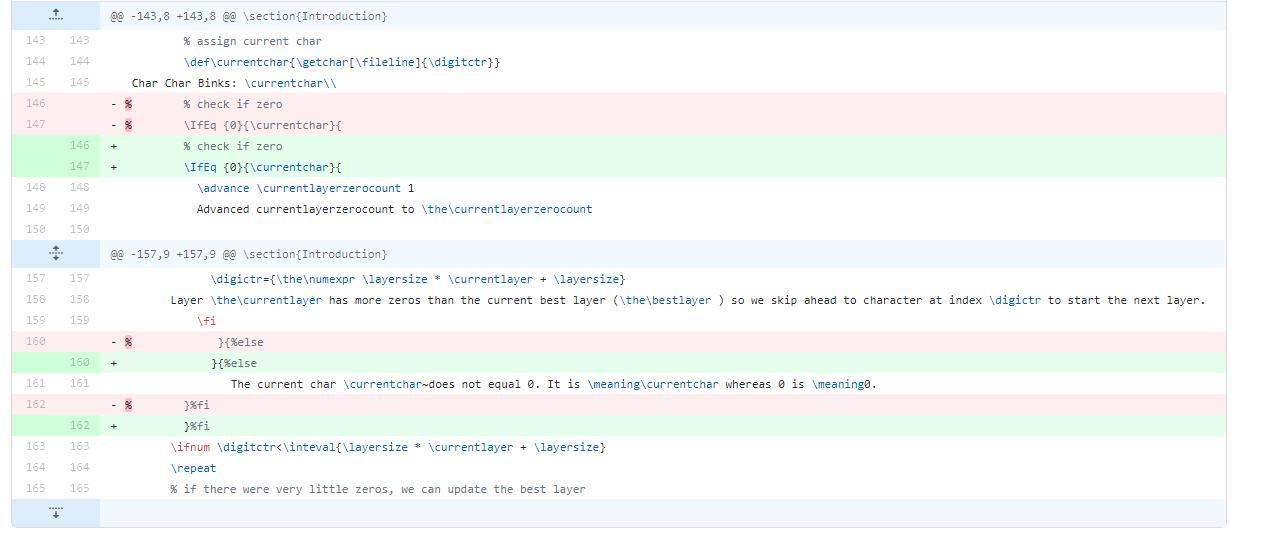
\includegraphics[width=1.6\textwidth]{diff}}%
  \caption{The difference between wrong code that compiles (red) and seemingly correct code that produces a compiler error (green).}
  \label{fig:diff}
\end{figure}

Finally, the performance of the \texttt{xstring} package is whack. It takes more than two minutes to figure out the length of a 15'000 character string. The bash command \texttt{wc -c inputfile.txt} does that in less than a second.
\clearpage
\section{StrLen}
Since \texttt{xstring}'s \texttt{StrLen} is so slow, how about creating a faster one?
We'll just have to run tex with the \texttt{--shell-escape} flag.\citelist{\cite{shellescape}} ( See \autoref{fig:typesettingsettings}). Using that allows us to escape to the shell - which is either bash or the windows cmd.exe.

\begin{figure}[htbp]
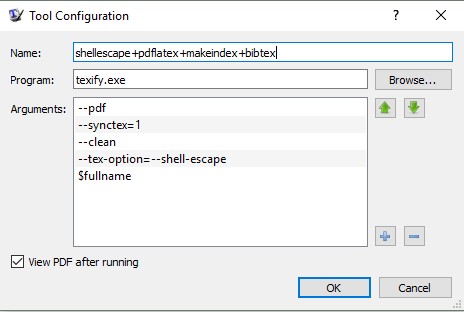
\includegraphics{typesettingsettings}
\caption{TeXworks settings for shellescape}
\label{fig:typesettingsettings}
\end{figure}

%\immediate\write18{wc -c inputfile.tex > scriptoutput.tex}
%Character Count: \input{scriptoutput.tex}
A simple \texttt{\textbackslash input\{|"echo test"\}} already works!
\input{|"echo test!"}

But I cannot figure out how to correctly call \texttt{wc -c inputfile.tex} because the shell spawns in the wrong path. And also, for some reason the following code does not even create a file \texttt{outfile.blubb} anywhere on my machine.
\begin{lstlisting}
\input{|"echo a > outfile.blubb"}
\end{lstlisting}
The problem seems to be, according to the logs, that the pipe closes before the left side is finished writing to stdout. But that is actually happening due to the \texttt{echo} earlier. When I leave it out, that's not logged.

Maybe using python is easier? You'd have to read the source to get this one though.\citelist{\cite{pythonescape}}
\begin{lstlisting}
\begin{pycode}{abc}
print(1+12)
\end{pycode}
\end{lstlisting}
But no, that also results in a problem with writing to a file... So let me try something I understand!
\begin{mycode}
\input{|"python -c "print(1+2);""}
\end{mycode}
\typeout{trying python}
\input{|"python -c "print(1+2);""}
\newline
And as you should be able to see, it works!

So for computing stringlength, a quick python call should speed things up.
\begin{mycode}
\input{|"python -c "print(len('mystringofunkownlength'));""}
\end{mycode}
\input{|"python -c "print(len('mystringofunkownlength'));""}
\newline
It is notable that spaces within that string get lost before they are passed to python. Thankfully we don't need this here. But this reminds my of \href{https://ctftime.org/writeup/21982}{PyAuCalc}.

We can make \LaTeX\, paste a string into that as well...

\begin{mycode}
\def\mystr{hello}
\def\mystrtwo{\mystr}
\input{|"python -c "print(len('\mystrtwo'));""}
\end{mycode}
\def\mystr{hello}
\def\mystrtwo{\mystr}
\input{|"python -c "print(len('\mystrtwo'));""}
...but for some reason it fails when used with our included inputstring. There's a site with an example on how to include text from a file, but it does not work at all for me\citelist{\cite{stackexpand}}. I guess I'll just hardcode it inside this file here instead... For that, however, the line length limit becomes an issue. So I've declared 74 commands and combined them into one. Aand turns out that also didn't help. The string just ends after some two hundred characters.

So to quote a professor of mine, J. Hromkovic, \textit{"\textbf{Strategy: We Give Up!} What can we do to still be able to state something impressive?"}.
Well, I can just hardcode the damn string length. That's not really worse than hardcoding the input.

\makeatletter
\def\einput#1{\@@input #1 \space}
\newcommand{\showexpanded}[1]{%
  \everyeof{\expandafter\@gobble\noexpand}%
  \long\edef\@tempcontents{#1}%
  \show\@tempcontents
}
\newcommand{\justexpanded}[1]{%
  \everyeof{\expandafter\@gobble\noexpand}%
  \long\edef\@tempcontents{#1}%
  \@tempcontents
}
\makeatother
\def\testingfile{\einput{testing.tex}}
%\showexpanded{\testingfile}
%\justexpanded{\testingfile}
%\input{|"python -c "print(len('\hardcodedinput'));""}
%\hardcodedinput

\section{Get Head Performance}
Again, \texttt{xstring} is extremely slow with big strings. So I split everything into layers of 100 chars. But that's still noticeably slower at the end of the layer than at the start of the layer... even though it's only supposed to be a quick character access. So I'm transforming everything into head accesses at index zero.

\section{Scoping}
Nested loops require scoping around the inner loop. Which in turn means we need to use the \verb!\global!  keyword to assign to variables from outside the inner scope. And that in turn makes it really weird to use \texttt{StrGobbleLeft} from the \texttt{xstring} package when I'm trying to remove a character and store the result back in the same string.

The solution is probably a rewrite that uses only one loop plus an if condition that checks the modulus of the loop counter and acts appropriately whenever a layer is finished.

\section{Execution: Getting our Feet Wet}

We had \Strawberries\ Strawberries for this year's harvest. Probably not enough.
So we are sad now and solve https://adventofcode.com/2019/day/8.

% get first character of string hello
\getchar[hello]{1}
\getcoolchar[hello]{2}
%\firstchar{122222222021222212220220022122202222022012222222222222022022122222220210000222222222222112222222222022222222222222222222222222022022222222222222222222022222222220222202120221122222212222122202222222222222022222222222222210010222222222222202222222222022222222222222222222222222022222222222222222222222022222222222222212021221222222212222222002222222222222022022022222221201000222222222222202222222222122222222222222222222222222122222222222222222222222122222222122222202022220222022222222122102222222222222122222222222220202202222222222222012222222222222222222222222222222222222222122222222222222222222222222222222222222122222022002212222222002222222222222122022122222221210200222222222222122222222222022222222222222222222222222022022222222222222221222022222222222122212121220222122202222122022222222222222122022222222221222212222222222222202222202222022222222222022222222222222222122222222222222222222222222222222222222121222222102222222222212222222222222222022022221221201212222222222222122202212222122222222222022222222222222122222222222222222222222122222222222222222122222222222202222022122222222222222122222022220220211010222222222222202212202222122222222222022222222222222022022222222222222220222122222222020222222020222022102202222122212222222222222222122022220211220210222222222222202222212222122222222222022222222222222222022222222222222221222122222222122122212021221122212212222022002222222222222222022022222212202020222222222222122222212202122222222222122212222222222122222222222222222222222222222222121122212020221022112202222022122222222222222022022122220202221220222222222222012202212222222222222222022222222222222222122222222222222221222222222222222122202220221022102222222222012222222222222222120122222202200210222222222222222222202212022222222222122202222222222222222222022222222220222222222222220222202020220222122222222222102222222222222122122022220210220122222222222220012212222222222222222222222222222222222222122222022222222221222022222222122222222120221222000202222222222202222222222222021122221202200011222222222222002202202212222222222222122202222222222022122222022222222220222122222222022222202020221122201202222022112212222222222022020022221201210021222222222220002202202212022222222222122202222222222122022222022222222222222022222222022222202221221022111202202222122222222222222122221122221221210200222222222222002222222212122222222222022212222222222122222222222222222220222122222222020122222122222222102212212122212202222222222122020022221201220120222222222220202222212202222222222222022212222222222222122222122222222220222022222222021022222221221022112202202122202212222222222122020122220202221010222222222221122212212222122222222222222222222222222122222222222222222221222122222222221022202222222222022222212122112222222222222022022222220210221220222222202220002222212222122222222222122222222222222022222222122222222220222222222222220222202121220022122222212122122202222222222122222222221202201022222222222221222202222222122222222222222212222222222122222222022222122222222222222222221222202121220022010222202022112222222222222122021122222211211221222222202222202222202222122222222222022222222222222122022222122222222220222122222222220220222120221222012222222222202202222222222222221022220201211222222222212220012202222212022222222222222202222222222022222222122222222221222022222222222120212022220022000202222022122212222222222022022022221222200210222222212221212202212222222222222222122212222222222022122222022222022221222122222222020022222120221022121112222122102212222222222222021022220212202011222222202220012202202212222222222222222212022222222022022222222222022222222022222222220020202121220022112022202022022222222222222222221022220210210110222222222220102202202222222222222222022212022222222122022222222222122220220022222222221021212121220022122222212222112202222222222122121222222211200210222222222221002212212202022222222222022212222220222222222222122222022221222022222222122220212221220222010222122122122202222222222222121122221212220100222222222220122202212212222222222222122222122202222021222222122222022222221022222222222021222120222122112002202122022212222222220022222222220212202222222222212220012212212222122222222222022222122220222022222222122222222220221222222222120221212221221222221212022222212222222222221222220222222201212100122222202221022202222202022222222222122222022220222120022222122222222221222022220222122220212222220222211002102222012202222222221022122122220221202122122222202222222212212222022222122222122202122211222020222222022222022221221222222222121120222022222222101002122022222212222222222222120022220212211112022222222222112212212212122222022222122222222210222121022222122222122222220122220212222121202021222212202212122222102222222222220022221122221212220211122222212221022212202212022222122222022202022200222020222222222222122221221122220222122021222120222012200112102122212212222222221122022122221220222121222222222220222222212202122222222222122202122211222222122222022222222221222022220212121220212020221202220012022222222202222222221022222022220221202102222222222222222222222212122222122222222222002211222121122222222222222221222222220222221120212220222122212202012022022222222222222122220222220200221101222022202221122202202202022222022222222212212201222120022222022222122222220222221212022021202221222002001112012122212202222222222222122122220201200122122022212221222222202202222222222222122212222200222022022222022222022220222222220212022220202121220212201202022022112222222222222122021122222221202220122122202220112212212222122222222222022202022222222120122222022222222221222022222222021121202221220122201212022122222222222222220122120022222221211001122222212222222212212202122222022222122202012220222121222222122222122220221022222202122120202120221002120202212122022202222222220122221022221221212222022022202220002212202212222222222222222222212200222122122222022222122221221022221202022221202022222112000112102222222202222222222022022222222210202212222122212220012222222212222222222222022222212222222222022222222222022220220022220212121220212022221102111222002222112202222222222222222022220221211012122222222221002202202222122222222222022202202221222222122222222222222221220022222212021122202222220002011202022222102222222222220122020022221200201010222222222222122202202202022222222222222222122221222020122222022222222221202122222212022020202121222112102112122022212222222222220022020122222211221011222222222221012222222222122222222222222202112212222022022222022222122222220022122202220122102022220012012122112022122222222222221222022022220220201211221122202222222212202212122222022222222222122200222120222222022222122222200122122202222121012122221202010212202122122202222222222222122102222220202121021022222221112202222202022222002222122212102210222121222222022222122221220222020222122022122120220212202002022222222202222222222222120102221222212210020022222222202202202222222222112222022202122211222021022222222222122220220122122212220220122220221202110122012022212212222222221222122222220212202222022122222210022202212202122222022222022212122210222022022222122222222222210022120202020021122121220222222022002122022212222222221122122002222222220111220122212202102222202222122222012222022202112201202020122222022222022221221022120202221120002121221222122002222122112202222222222022222012221202210222020122222212202202222222122222012222122202012220212222222222022222222221211222022202220122222121222002121212202222102212222222222022121122221211201100221122222211212222212212122222122222122222222201202020122222122222022220220022222202122220102121222122210202212122202202222222222122220002222210211100020122212200212212222202022222122222222212102200222021022222222222022221211022220222022000022022222112102102022022122212222222222022222222220201211222020222222222112202222202122222122222222202022211202022222222022222122221210222121202022001212222220102222222212122102212222222221222120202222200200120021122212222102212202202222222102222022212022210202220022202022222122221201220120222022220202020222102202102102122012222222222221022221102221200212100121122222202022212222212122222002222122222122220202122222222122222222222221221022212122012222021222002120102112222112222222122220122220022222202211102220222202221102212222212222222102221122222112221222021222212122222022222221121022212222221022220221102020222002222122222222122222022020012221200210110020122212221002212212212222222202221222202022212212120122212021222122221220221120212022022112222221222112212012122222222222222222122021202220200212022020222222212122202222202122222122221022222002212202120022202122222122222212120122202021201022220221102220122002022010222222122221122221112221222222020122022202210222202222212022222002222222212202211202120222102122222222221202022020212122011222121221002011102112222012212222222222122020012222200212222020022212222202212202222022222122220022202202222202120222012120222122221210022020222120211012022222002001212102022102202222122222022121122221210210121022222202222102202202202222222200220122202122200212021021122021222222220200221221202221001212020222112110002122222120222222222222022222212221222220201121022222202202222202222220222122221122212202201202220021002222222122221201122200222222220122022221222102202212022212212222002221222221122222200202012022102212200012202222212221222201221122222012221212022121002121222222220221121020212021110202121222022222102222022220212220002221222221202221222221112121112202012222212202202122222222222022212202220202022122112020222122221221021111212122211112221221002021122222122210212220022221122121102222211222121020122202212112222212222022222012221022222200201212020122022221222122221220122202202021201112121221112200012112022111222122012221122120012221222222110120122212111222202212202120222211221122202020212222221021122020222222220200020112212121121002220221102122022212222201202220122220122221222222201222222221022212002122212222202021222112221022222001200202120221112021222122221211122222202122010122020222122211002212022102202122112222222120022220221211120221202212200102222212202220222200220122202112210222122120102020222022220222221002222121011202120221022220222022122200212222002222122221212221222211101021012222201012222212202022222122220222202100220222222122122021222122220202022212202122000112022220202201222121122222212220002222122120110220200211022121122222000222212212222221222010220222222120201222022121222122222022221220221020212020202222220221212110122210222001212021212222022122211222210212010220112212210012222222220222222121222222212202202222121220222021222122222212222102212122111122221220122112202122022211202022022220122221112222211220221022112212000012210222220020222100220222000212201212121121020021222222220212121112202202121222120220112211002002222022202221222220222222211222112222010221122212022102201212221022222101221022222211212202121221012120222022221220022012202222122022122210202011222211022001222202002222122221222221101201021120002222212122200202221120222020222222101021200222220020122220222122222202122120202101201022122200112022022201222111222011122220222221110220222210001221002202201022200212210221222020221022122220200202221121101121222022220220022001102002002102022222102101202212022202202221112220022222020220211201121020012222202212221202222021222201220222121201210222020121021221222122220221120122122222201102122212122002012112122012212020222220122220221221201201222101202212202202211212222022222112220222202201212202221022002122222122221202100011112102200212020202102102212121022121202000022221122121012222002220000002011202001112211222211021222102222122110101221222020020102222222022222212120011002112021122021210222222212110222121222010122222122022202220211212020010201222010112201202222122222020220022221001210212222021211022222222222211010002212122222112121221102110012120022201202102212221122122212220020212201001120222011002221022210121222220221022220021222202220220112122222022221222010222202102010102222200212011122210221212222222002220122022110222220200212220002222202022221222202021222022221122112121221222020021002121222222222222202110202102112122020200122000112000122122212211202220222021212221200210220221010222222002202212220121222122222222100020211221021221211022222222221222112101002202222212220200122002122200222100202111222220222120020222020200121010001222201112202202200221222212221022210212212222122222022121222022222110101021102112002012022202022202002010020102202221022220122022201221210212002011212222122122201222220221120012222122012220210202021220010020222022221110212210202021220202220202112002122220121221222212012220222121102221202212101201102202011112200022222021022220221122002211221222021021110021222222220201211120112002011012122201102021022222020100212022112221020122212220021221201102022222121202220102202020121002222002110121220221222022122022222222222121211112222122220002220212002121202221120022202222022222022021221221112202212112111222010212212002201222220202220102010221102210120221101222222222221102002012012120022122120210202222212022122210222200212222121220112222220202021201212222201222211202220221122221221122212202010222020120120122222022221100220212102100001002021212002111112001120212222122012220122021012221001211210222221202220212222122202020022121220002000112102201220021101120222222221101011200022121121212020210112201002012222221212002102120121020020221000210221011012222210122222222200022221111221212020210000222022120212021222022220202112010202000012022220212202000202212121001212212012221220020222220221202111222010002022112222122211121020211222222200101111222020121120022222222220111001011212020000012220202022022112011221102002020122221022122111222100200021011010222100102212112221221222112220122111111211200020100221120222222221001212110112201002102002222222211022220020121222122012120011220022221200201101011211122112102211222202221122202222002200210222200021000211122222112220011000101112000122002102202022001222102221001102122122021022020200221112210000202021122111222202022200021200001201022002110100212122011121120222012220010022002122022210022111210212202002001102212102121022021111221200220022201210121010122110222221212212021010102222102002220221210122110120120222102222111122100112202211112021120012122102212011211122102022220002220221221120211211101200212002102220112221222020220201122011020012221220101002020222122220100221011122120000212101002102100122110000110012200002221021122022220221201020000211112112112212222210120000000201102200210110212221101210022222202220020112002022021022122021010222121222120021101222022202020120221022220112222201121122122010222222102220221211200210002211201012202022112212020122002220220100112202122002102122010122210022200100011222101212220211020111220222222001122120102221212221222210122012020202122020101001211120200100120022202221222011212202220000202001002002022202022110021220111202121222122122220201212200210220112002212212012210021002200212012111002001200121202200221022212221022000111200112220201120010120220220210222111022200001200222202210000100020021010101220200010122011000210212201122101121221121120101211021010101201000111
}

% compute integer arithmetic
\inteval{3 - 2}

% compute integer arithmetic
% "Although \relax does nothing by itself, it is a safe command to stop expansion of another command"
\newcommand\three{3}
\the\numexpr \three - 2 + 5 \relax
% and to store it in a variable???? redirection and then reusing \three does not work. We need a new variable.
\def\tmp{\three}
\def\four{\the\numexpr \tmp - 2 + 5 }

\newcommand\threehundred{300}

% include the input file
\ifdebug
  \def\inputstring{220002201222100002
}
  \def\inputstringlength{19}
\else
  \def\inputstring{122222222021222212220220022122202222022012222222222222022022122222220210000222222222222112222222222022222222222222222222222222022022222222222222222222022222222220222202120221122222212222122202222222222222022222222222222210010222222222222202222222222022222222222222222222222222022222222222222222222222022222222222222212021221222222212222222002222222222222022022022222221201000222222222222202222222222122222222222222222222222222122222222222222222222222122222222122222202022220222022222222122102222222222222122222222222220202202222222222222012222222222222222222222222222222222222222122222222222222222222222222222222222222122222022002212222222002222222222222122022122222221210200222222222222122222222222022222222222222222222222222022022222222222222221222022222222222122212121220222122202222122022222222222222122022222222221222212222222222222202222202222022222222222022222222222222222122222222222222222222222222222222222222121222222102222222222212222222222222222022022221221201212222222222222122202212222122222222222022222222222222122222222222222222222222122222222222222222122222222222202222022122222222222222122222022220220211010222222222222202212202222122222222222022222222222222022022222222222222220222122222222020222222020222022102202222122212222222222222222122022220211220210222222222222202222212222122222222222022222222222222222022222222222222221222122222222122122212021221122212212222022002222222222222222022022222212202020222222222222122222212202122222222222122212222222222122222222222222222222222222222222121122212020221022112202222022122222222222222022022122220202221220222222222222012202212222222222222222022222222222222222122222222222222221222222222222222122202220221022102222222222012222222222222222120122222202200210222222222222222222202212022222222222122202222222222222222222022222222220222222222222220222202020220222122222222222102222222222222122122022220210220122222222222220012212222222222222222222222222222222222222122222022222222221222022222222122222222120221222000202222222222202222222222222021122221202200011222222222222002202202212222222222222122202222222222022122222022222222220222122222222022222202020221122201202222022112212222222222022020022221201210021222222222220002202202212022222222222122202222222222122022222022222222222222022222222022222202221221022111202202222122222222222222122221122221221210200222222222222002222222212122222222222022212222222222122222222222222222220222122222222020122222122222222102212212122212202222222222122020022221201220120222222222220202222212202222222222222022212222222222222122222122222222220222022222222021022222221221022112202202122202212222222222122020122220202221010222222222221122212212222122222222222222222222222222122222222222222222221222122222222221022202222222222022222212122112222222222222022022222220210221220222222202220002222212222122222222222122222222222222022222222122222222220222222222222220222202121220022122222212122122202222222222122222222221202201022222222222221222202222222122222222222222212222222222122222222022222122222222222222222221222202121220022010222202022112222222222222122021122222211211221222222202222202222202222122222222222022222222222222122022222122222222220222122222222220220222120221222012222222222202202222222222222221022220201211222222222212220012202222212022222222222222202222222222022222222122222222221222022222222222120212022220022000202222022122212222222222022022022221222200210222222212221212202212222222222222222122212222222222022122222022222022221222122222222020022222120221022121112222122102212222222222222021022220212202011222222202220012202202212222222222222222212022222222022022222222222022222222022222222220020202121220022112022202022022222222222222222221022220210210110222222222220102202202222222222222222022212022222222122022222222222122220220022222222221021212121220022122222212222112202222222222122121222222211200210222222222221002212212202022222222222022212222220222222222222122222022221222022222222122220212221220222010222122122122202222222222222121122221212220100222222222220122202212212222222222222122222122202222021222222122222022222221022222222222021222120222122112002202122022212222222220022222222220212202222222222212220012212212222122222222222022222122220222022222222122222222220221222222222120221212221221222221212022222212222222222221222220222222201212100122222202221022202222202022222222222122222022220222120022222122222222221222022220222122220212222220222211002102222012202222222221022122122220221202122122222202222222212212222022222122222122202122211222020222222022222022221221222222222121120222022222222101002122022222212222222222222120022220212211112022222222222112212212212122222022222122222222210222121022222122222122222220122220212222121202021222212202212122222102222222222220022221122221212220211122222212221022212202212022222122222022202022200222020222222222222122221221122220222122021222120222012200112102122212212222222221122022122221220222121222222222220222222212202122222222222122202122211222222122222022222222221222022220212121220212020221202220012022222222202222222221022222022220221202102222222222222222222222212122222122222222222002211222121122222222222222221222222220222221120212220222122212202012022022222222222222122220222220200221101222022202221122202202202022222022222222212212201222120022222022222122222220222221212022021202221222002001112012122212202222222222222122122220201200122122022212221222222202202222222222222122212222200222022022222022222022220222222220212022220202121220212201202022022112222222222222122021122222221202220122122202220112212212222122222222222022202022222222120122222022222222221222022222222021121202221220122201212022122222222222222220122120022222221211001122222212222222212212202122222022222122202012220222121222222122222122220221022222202122120202120221002120202212122022202222222220122221022221221212222022022202220002212202212222222222222222222212200222122122222022222122221221022221202022221202022222112000112102222222202222222222022022222222210202212222122212220012222222212222222222222022222212222222222022222222222022220220022220212121220212022221102111222002222112202222222222222222022220221211012122222222221002202202222122222222222022202202221222222122222222222222221220022222212021122202222220002011202022222102222222222220122020022221200201010222222222222122202202202022222222222222222122221222020122222022222222221202122222212022020202121222112102112122022212222222222220022020122222211221011222222222221012222222222122222222222222202112212222022022222022222122222220022122202220122102022220012012122112022122222222222221222022022220220201211221122202222222212202212122222022222222222122200222120222222022222122222200122122202222121012122221202010212202122122202222222222222122102222220202121021022222221112202222202022222002222122212102210222121222222022222122221220222020222122022122120220212202002022222222202222222222222120102221222212210020022222222202202202222222222112222022202122211222021022222222222122220220122122212220220122220221202110122012022212212222222221222122222220212202222022122222210022202212202122222022222022212122210222022022222122222222222210022120202020021122121220222222022002122022212222222221122122002222222220111220122212202102222202222122222012222022202112201202020122222022222022221221022120202221120002121221222122002222122112202222222222022222012221202210222020122222212202202222222122222012222122202012220212222222222022222222221211222022202220122222121222002121212202222102212222222222022121122221211201100221122222211212222212212122222122222122222222201202020122222122222022220220022222202122220102121222122210202212122202202222222222122220002222210211100020122212200212212222202022222122222222212102200222021022222222222022221211022220222022000022022222112102102022022122212222222222022222222220201211222020222222222112202222202122222122222222202022211202022222222022222122221210222121202022001212222220102222222212122102212222222221222120202222200200120021122212222102212202202222222102222022212022210202220022202022222122221201220120222022220202020222102202102102122012222222222221022221102221200212100121122222202022212222212122222002222122222122220202122222222122222222222221221022212122012222021222002120102112222112222222122220122220022222202211102220222202221102212222212222222102221122222112221222021222212122222022222221121022212222221022220221102020222002222122222222122222022020012221200210110020122212221002212212212222222202221222202022212212120122212021222122221220221120212022022112222221222112212012122222222222222222122021202220200212022020222222212122202222202122222122221022222002212202120022202122222122222212120122202021201022220221102220122002022010222222122221122221112221222222020122022202210222202222212022222002222222212202211202120222102122222222221202022020212122011222121221002011102112222012212222222222122020012222200212222020022212222202212202222022222122220022202202222202120222012120222122221210022020222120211012022222002001212102022102202222122222022121122221210210121022222202222102202202202222222200220122202122200212021021122021222222220200221221202221001212020222112110002122222120222222222222022222212221222220201121022222202202222202222220222122221122212202201202220021002222222122221201122200222222220122022221222102202212022212212222002221222221122222200202012022102212200012202222212221222201221122222012221212022121002121222222220221121020212021110202121222022222102222022220212220002221222221202221222221112121112202012222212202202122222222222022212202220202022122112020222122221221021111212122211112221221002021122222122210212220022221122121102222211222121020122202212112222212222022222012221022222200201212020122022221222122221220122202202021201112121221112200012112022111222122012221122120012221222222110120122212111222202212202120222211221122202020212222221021122020222222220200020112212121121002220221102122022212222201202220122220122221222222201222222221022212002122212222202021222112221022222001200202120221112021222122221211122222202122010122020222122211002212022102202122112222222120022220221211120221202212200102222212202220222200220122202112210222122120102020222022220222221002222121011202120221022220222022122200212222002222122221212221222211101021012222201012222212202022222122220222202100220222222122122021222122220202022212202122000112022220202201222121122222212220002222122120110220200211022121122222000222212212222221222010220222222120201222022121222122222022221220221020212020202222220221212110122210222001212021212222022122211222210212010220112212210012222222220222222121222222212202202222121220222021222122222212222102212122111122221220122112202122022211202022022220122221112222211220221022112212000012210222220020222100220222000212201212121121020021222222220212121112202202121222120220112211002002222022202221222220222222211222112222010221122212022102201212221022222101221022222211212202121221012120222022221220022012202222122022122210202011222211022001222202002222122221222221101201021120002222212122200202221120222020222222101021200222220020122220222122222202122120202101201022122200112022022201222111222011122220222221110220222210001221002202201022200212210221222020221022122220200202221121101121222022220220022001102002002102022222102101202212022202202221112220022222020220211201121020012222202212221202222021222201220222121201210222020121021221222122220221120122122222201102122212122002012112122012212020222220122220221221201201222101202212202202211212222022222112220222202201212202221022002122222122221202100011112102200212020202102102212121022121202000022221122121012222002220000002011202001112211222211021222102222122110101221222020020102222222022222212120011002112021122021210222222212110222121222010122222122022202220211212020010201222010112201202222122222020220022221001210212222021211022222222222211010002212122222112121221102110012120022201202102212221122122212220020212201001120222011002221022210121222220221022220021222202220220112122222022221222010222202102010102222200212011122210221212222222002220122022110222220200212220002222202022221222202021222022221122112121221222020021002121222222222222202110202102112122020200122000112000122122212211202220222021212221200210220221010222222002202212220121222122222222100020211221021221211022222222221222112101002202222212220200122002122200222100202111222220222120020222020200121010001222201112202202200221222212221022210212212222122222022121222022222110101021102112002012022202022202002010020102202221022220122022201221210212002011212222122122201222220221120012222122012220210202021220010020222022221110212210202021220202220202112002122220121221222212012220222121102221202212101201102202011112200022222021022220221122002211221222021021110021222222220201211120112002011012122201102021022222020100212022112221020122212220021221201102022222121202220102202020121002222002110121220221222022122022222222222121211112222122220002220212002121202221120022202222022222022021221221112202212112111222010212212002201222220202220102010221102210120221101222222222221102002012012120022122120210202222212022122210222200212222121220112222220202021201212222201222211202220221122221221122212202010222020120120122222022221100220212102100001002021212002111112001120212222122012220122021012221001211210222221202220212222122202020022121220002000112102201220021101120222222221101011200022121121212020210112201002012222221212002102120121020020221000210221011012222210122222222200022221111221212020210000222022120212021222022220202112010202000012022220212202000202212121001212212012221220020222220221202111222010002022112222122211121020211222222200101111222020121120022222222220111001011212020000012220202022022112011221102002020122221022122111222100200021011010222100102212112221221222112220122111111211200020100221120222222221001212110112201002102002222222211022220020121222122012120011220022221200201101011211122112102211222202221122202222002200210222200021000211122222112220011000101112000122002102202022001222102221001102122122021022020200221112210000202021122111222202022200021200001201022002110100212122011121120222012220010022002122022210022111210212202002001102212102121022021111221200220022201210121010122110222221212212021010102222102002220221210122110120120222102222111122100112202211112021120012122102212011211122102022220002220221221120211211101200212002102220112221222020220201122011020012221220101002020222122220100221011122120000212101002102100122110000110012200002221021122022220221201020000211112112112212222210120000000201102200210110212221101210022222202220020112002022021022122021010222121222120021101222022202020120221022220112222201121122122010222222102220221211200210002211201012202022112212020122002220220100112202122002102122010122210022200100011222101212220211020111220222222001122120102221212221222210122012020202122020101001211120200100120022202221222011212202220000202001002002022202022110021220111202121222122122220201212200210220112002212212012210021002200212012111002001200121202200221022212221022000111200112220201120010120220220210222111022200001200222202210000100020021010101220200010122011000210212201122101121221121120101211021010101201000111
}
  \def\inputstringlength{15000}
\fi
% and print it
\inputstring

% include the input file in a different way because the previous way fails when passed as argument to getchar
\ifdebug
\newread\file
\openin\file=debuginputfile.tex
\read\file to \fileline
\closein\file
\else
\newread\file
\openin\file=inputfile.tex
\read\file to \fileline
\closein\file
\fi

hello world 
% get second character of inputfile
\getchar[\three]{1}
\getcoolchar[300]{1}
\getcoolchar[\threehundred]{1}
\typeout{===>"three"|\three}

% Variables given by the task
\newcount{\imgwidth}
\imgwidth=25
\newcount{\imgheight}
\imgheight=6
\ifdebug
\imgwidth=3
\imgheight=2
\fi

Image Width: \the\imgwidth \hspace{1cm}Image Height: \the\imgheight

% compute size of a layer
\newcount{\layersize}
\layersize=\the\imgwidth
\multiply\layersize by \imgheight \relax
\typeout{Size of a layer is \the\layersize}
I want to loop \the\layersize~times for the first layer.

% store the index of the best layer. The best layer has the fewest digits. So initialize the counter to maximum possible + 1.
\newcount\bestlayer
\bestlayer=-1
\newcount\bestlayerzerocount
\bestlayerzerocount=\inteval{\layersize + 1}
\global\newcount\currentlayerzerocount
\newcount\currentlayer

% now for the first layer count the number of zeros
\currentlayer=0
\currentlayerzerocount=0
\global\newcount\digitctr
\digitctr=0 % count from 1, not from zero. So we count from 1 to \layersize because we start advancing at the start of the loop.
% TODO: optimize getting current char by deleting from string.
%
\newcount\layerafterthelast

%%\StrLen{\fileline}[\stahp]%find the strlen and store it in \stahp
%% see https://tex.stackexchange.com/a/15424/102826
\def\stahp{\inputstringlength}

\def\stahpnow{\the\numexpr \stahp - 1}

The input file contains \stahpnow characters.

%ifrunpartone
\ifrunpartone
\section{ Execution: The Water Is Cold}
\begin{myquote}\begin{quote}
\texttt{\textbackslash global} is a TeX command that declares the following definition or assignment to be global, meaning that if TeX is currently inside a group, the definition or assignment will still remain valid when the group is over. Commands that can follow \texttt{\textbackslash global} include \texttt{\textbackslash def}, \texttt{\textbackslash edef}, \texttt{\textbackslash let}, \texttt{\textbackslash count}, \texttt{\textbackslash countdef}, [...]\citelist{\cite{wikibooksglobal}}\\
\end{quote}\end{myquote}
An alternative to using globals would be to use tikz loops with the \texttt{remember} option \citelist{\cite{tikzremember}}. Another option I see is using counters instead of counts - they are the latex version of the tex counter. For counters, you can apparently not use \texttt{\textbackslash the \textbackslash ctr}, you have to use\texttt{\textbackslash thectr} (See \autoref{c:simpleLoop}).
\begin{figure}
\begin{mycode}
\newcounter{outerloopcounter}
\setcounter{outerloopcounter}{0}
\loop
    	\addtocounter{outerloopcounter}{1}
           \theouterloopcounter ,
           \ifnum \value{outerloopcounter}<3
\repeat
outerloopcount: \theouterloopcounter
\end{mycode}
\caption{Simple Loop using TeX Counters}
\label{c:simpleLoop}
\end{figure}

Now let us do the same thing again, but with nested loops. See \autoref{c:nested}.
\begin{figure}[htbp]
\begin{mycode}
\newcounter{outerloopcounter}
\setcounter{outerloopcounter}{0}
\newcounter{innerloopcounter}
\loop
	\setcounter{innerloopcounter}{0}
    	\addtocounter{outerloopcounter}{1}
	
	{\loop
	\addtocounter{innerloopcounter}{1}
           (\theouterloopcounter , \theinnerloopcounter )
	\ifnum \value{innerloopcounter}<2
           \repeat }

           \ifnum \value{outerloopcounter}<3
\repeat
outerloopcount: \theouterloopcounter
\end{mycode}
\caption{Nested Loops using LaTeX Counters}
\label{c:nested}
\end{figure}
That requires curly braces around the inner loop. Otherwise, only the first outer loop iteration is run.

For the actual implementation, we assume that we are given \texttt{inputstringlength}, \texttt{imgwidth}, and \texttt{imgheight}. Computing those from the input string is feasible but takes long.

I'm using an \texttt{edef} to overwrite the \texttt{workingline} variable every loop.

% optimization because xstring library is slow.
% We remove the head of the input string once it has been used. This happens every time the layer has been read.
\def\workingline{\fileline}
%
\newcounter{layercounter}
\setcounter{layercounter}{0}
\newcounter{charinlayercounter}
\bigskip\noindent
\def\numlayers{\the\numexpr \inputstringlength / \layersize \relax}
Computation starting with \numlayers ~ Layers of size \the\imgwidth x\the\imgheight.
\newcounter{currentlayerzerocounter}\setcounter{currentlayerzerocounter}{0}
\newcounter{bestlayercounter}\setcounter{bestlayercounter}{0}
\newcounter{bestlayerzerocountcounter}\setcounter{bestlayerzerocountcounter}{\the\numexpr \layersize}
\newcounter{currentcharpos}\setcounter{currentcharpos}{\the\numexpr 0 - 1}
\newcounter{charstoremoveatendoflayer}\setcounter{charstoremoveatendoflayer}{0}

Normally, I would do a first loop for finding the best Layer and a second block for extracting the relevant information. However, given that the loops are so slow with all those string operations, I'll just spend some brain overhead and do this in one loop, even if it is a bit harder to keep the overview.\\

\newcounter{bestlayeronedigitscounter}
\newcounter{bestlayertwodigitscounter}
\newcounter{currentlayeronecounter}
\newcounter{currentlayertwocounter}

% loop through all layers
\loop
	% reset counters to start of layer
	\setcounter{charinlayercounter}{0}
    	\addtocounter{layercounter}{1}
	\setcounter{currentlayerzerocounter}{0}
	\setcounter{currentlayeronecounter}{0}
	\setcounter{currentlayertwocounter}{0}
	\setcounter{charstoremoveatendoflayer}{1}
	
	{\loop % loop through all characters in the current layer
	\addtocounter{charinlayercounter}{1}
	\addtocounter{currentcharpos}{1}
	\ifverbose
           (\thelayercounter , \thecharinlayercounter )
	\fi

	% For each character in the current layer
		% assign current char as head
	             \StrMid{\workingline}{1}{1}[\currentchar]
		% check if zero
		\IfEq {0}{\currentchar}{
		  \ifverbose
		  The current char \currentchar~ equals 0.
		  \fi
		  \addtocounter{currentlayerzerocounter}{1}
		  % if current layer is worse than the best, no need to proceed checking
		  \ifnum \value{currentlayerzerocounter} > \value{bestlayerzerocountcounter}
			\ifverbose
			Skipping Layer \thelayercounter~ because it has more zeros than (i.e. it is worse than) Layer ~\thebestlayercounter.
			\fi
			% normally, one character will be removed, but now we need to remove all that are remaining in the layer
			\setcounter{charstoremoveatendoflayer}{\numexpr \layersize - \value{charinlayercounter}}
			% trigger stop condition at end of inner loop
			\setcounter{charinlayercounter}{\layersize}
		  \fi
		}{ % else
		  \ifverbose
		  The current char \currentchar~does not equal 0.\\
		  \fi
                       \typeout{Msg from IFEQ ELSE branch}
		} % fi

		% check if one
		\IfEq {1}{\currentchar}{
		  \addtocounter{currentlayeronecounter}{1}
		}{}

		% check if two
		\IfEq {2}{\currentchar}{
		  \addtocounter{currentlayertwocounter}{1}
		}{}

		 % truncate inputstring by one character at head
          		\typeout{about to remove \thecharstoremoveatendoflayer ~chars from head}
		\ifverbose
          		About to remove \thecharstoremoveatendoflayer ~chars from head
		\fi
           	\StrGobbleLeft{\workingline}{\value{charstoremoveatendoflayer}}[\workinglinetwo]
		\typeout{Reached character at position \thecurrentcharpos}
                	\global\edef\workingline{\workinglinetwo}

	\ifnum \value{charinlayercounter}<\layersize
           \repeat }

	% update best layer
	\ifnum \value{currentlayerzerocounter} < \value{bestlayerzerocountcounter}
		\ifverbose
		New Best Layer is Layer \thelayercounter.
		\fi
		\typeout{New Best Layer is Layer \thelayercounter}
		\setcounter{bestlayercounter}{\value{layercounter}}
		\setcounter{bestlayerzerocountcounter}{\value{currentlayerzerocounter}}
		\setcounter{bestlayeronedigitscounter}{\value{currentlayeronecounter}}
		\setcounter{bestlayertwodigitscounter}{\value{currentlayertwocounter}}
	\fi

           \ifnum \value{layercounter}<\numlayers
\repeat
\typeout{fFinished computation for Pt 1}
outerloopcount: \thelayercounter\\
Best Layer: \thebestlayercounter ~with \thebestlayerzerocountcounter ~zeros.\\
It has \thebestlayeronedigitscounter ~Ones and \thebestlayertwodigitscounter ~Twos.\\
\edef\res{\numexpr \value{bestlayeronedigitscounter} * \value {bestlayertwodigitscounter}}
This is a total of $n_\text{ones} \cdot n_{\text{twos}} = \the\res$.
\ifdebug

This result is from debug values.
\fi
%
%endif runpartone
\fi\typeout{"Reached the end of ifrunpartone"}

\section{Day Eight Part Two: Because this task wasn't that hard}
\typeout{"debug Srk 1!"}
\begin{myquote}\begin{quote}
Each image layer consists of numbers that represent pixel information. One digit, one pixel.
\begin{align*}
0 & \rightleftarrows \text{black}\\
1 & \rightleftarrows \text{white}\\
2 & \rightleftarrows \text{transparent}\\
\end{align*}
You're given multiple layers. For each pixel coordinate pair $(x, y)$ find the \textit{first} nontransparent value.
\end{quote}\end{myquote}
\typeout{"debug Srk9!"}
\ifrunparttwo
\typeout{"Starting the Lord's work!"}
\def\numlayers{\the\numexpr \inputstringlength / \layersize \relax}
\newcounter{charcounter}\setcounter{charcounter}{0}
\newcounter{layercounterx}
\newcounter{pixelvalue}
\def\workingstr{\fileline}
\loop
  \addtocounter{charcounter}{1}
  % for each pixel in the first layer, search all layers unti a pixel is opaque
           \setcounter{pixelvalue}{2}
	\setcounter{layercounterx}{-1}
	{\loop
	  \addtocounter{layercounterx}{1}
		\def\totalpos{\numexpr \value{charcounter} + ( \value{layercounterx} * \layersize )}
		\StrChar{\workingstr}{\totalpos}[\currentchar]
		\setcounter{pixelvalue}{\inteval{\currentchar}}
		\typeout{Considering Layer \thelayercounterx for pixel \thecharcounter}
		% if we reached the max layer and it's still 2, we keep the 2. But to abort the loop, we claim it's the magic number "minus one"
		\ifnum \value{layercounterx}=\inteval{\numlayers -1}
			\ifnum \value{pixelvalue}=2
				\setcounter{pixelvalue}{-1}
			\fi
		\fi
	  \ifnum \value{pixelvalue} > 1
	\repeat }
	% undo the hack from the inner loop:
	\ifnum \value{pixelvalue}=\inteval{0 - 1}
		\setcounter{pixelvalue}{2}
	\fi
	\typeout{Found \thepixelvalue in Layer \thelayercounterx for pixel \thecharcounter}
	\immediate\myappendxstring{\thepixelvalue}
\thepixelvalue
  \ifnum \value{charcounter} <  \layersize
\repeat
\else

\textbf{Not running part two as per flags.}

\fi

% perform some magic https://tex.stackexchange.com/questions/402173/append-strings-to-a-variable-and-display-them-at-the-front-of-the-document
Let me just perform some magic - Consider \autoref{fig:magic}. There's only one problem with that: It assumes that  the input strings are constant. Since I input the value of a counter, mine are not, and the magical string that ends up being collected is just a repetition of the last value it had. Adding \texttt{\textbackslash immediate} and \texttt{\textbackslash edef} was not helpful.\citelist{\cite{collectvar} \cite{immediatez}}

Now of course, I don't actually need that collection - I can place my computation wherever I like. It would still have been cool though - partly because I have weird spacing when I output my computation character by character, and partly because this is a nice trick to have in my spellbook at the ready. Luckily, the author of that trick replied to my inquiry by adding an \code{\textbackslash edef} and some \cprotect\code{\verb|\expandafter|} (\autoref{fig:segletes}).

\begin{figure}[hp]
\begin{myquote}
@lucidbrot
\begin{lstlisting}[columns=fullflexible, backgroundcolor = \color{codebggray}]
\def\myappendxstring#1{
  \edef\tmp{#1}\expandafter\g@addto@macro%
    \expandafter\mystring\expandafter{\tmp}
}\end{lstlisting}
Then, \begin{lstlisting}[columns=fullflexible, backgroundcolor = \color{codebggray}]
\stepcounter{mycounter} %
  \myappendxstring{Counter value is \themycounter. }
\end{lstlisting}
 - Steven B. Segletes 
\end{myquote}
\caption{S.B. Segletes' addition.}
\label{fig:segletes}
\end{figure}


% display the computed variable here
\makeatletter
\@starttoc{xyz}% executes stuff in .xyz file
\makeatother
Magic: \thefinalstring
% the following line must be performed at the end of the computation - e.g. at the end of the document.
\addtocontents{xyz}{\gdef\protect\thefinalstring{\mystring}}

\begin{figure}[htbp]
\begin{mycode}
% Throughout the document, collect the variable using
\myappendstring{hello}
% display the computed variable here
\makeatletter
\@starttoc{xyz}% executes stuff in .xyz file
\makeatother
\thefinalstring
% the following line must be performed at the end of the computation - e.g. at the end of the document.
\addtocontents{xyz}{\gdef\protect\thefinalstring{\mystring}}
\end{mycode}
\caption{Magic to collect a variable, then print it at the start of the document. \citelist{\cite{collectvar}}}
\label{fig:magic}
\end{figure}

\section{Todo}
Once this is done, I should inform the person who said I should inform them once this is done, to be found at \href{https://twitter.com/LucidBrot/status/1290792953548615682}{Twitter}.

I should probably also put the shellescape stuff into an optional branch. 

I want to attach the source code to this file.

I also want ot measure how long this takes.
\section{Performance}
%PDF Elapsed Time: \showthe\pdfelapsedtime
\begin{myquote}\begin{quote}
The value of \code{\textbackslash pdfelapsedtime} is the number of seconds elapsed multiplied by 65536. \citelist{\cite{robertson}}
\end{quote}\end{myquote}

\section{Source}
The source code is clingy: It attached itself to this file. Open it in Adobe Reader and view it under Attachments.\\
Linking to it does not work unless the file is also a pdf, it seems.

\begin{bibdiv}
\begin{biblist}
%\bib{Bourbaki70}{book}{
%title={Theorie des ensembles},
%author={Bourbaki, Nicolas},
%date={1970},
%publisher={Hermann},
%address={Paris}
%}
%\bib{Sokal96}{article}{
%title={Trangressing the boundaries},
%subtitle={Toward a transformative hermeneutics of quantum gravity},
%author={Sokal, Alan},
%journal={Social Text},
%volume={46/47},
%date={1996},
%pages={217--252}
%}
\bib{Gonzalo}{webpage}{
title={Nest StrLen and ifthenelse commands},
author={Medina, Gonzalo},
url={https://tex.stackexchange.com/a/15424/102826},
accessdate={05.08.2020}
}
\bib{shellescape}{webpage}{
title={texify.exe in TeXworks in MSWindows 10: MiKTex encountered internal error when compile with --shell-escape},
author={Desyllas, Dimitrios},
url={https://tex.stackexchange.com/a/437933/1028266},
accessdate={05.08.2020}
}
\bib{pythonescape}{webpage}{
title={Combining \LaTeX with Python},
author={Ziegenhagen, Uwe},
url={https://tug.org/tug2019/slides/slides-ziegenhagen-python.pdf},
date={09.08.2019},
accessdate={05.08.2020}
}
\bib{stackexpand}{webpage}{
title={Why is everyeof needed to avoid...},
author={Gross, Jason},
url={https://tex.stackexchange.com/q/516031/102826},
accessdate={07.08.2020}
}
\bib{wikibooksglobal}{webpage}{
title={TeX/global},
author={Burk},
url={https://en.wikibooks.org/wiki/TeX/global},
accessdate={21.08.2020}
}
\bib{tikzremember}{webpage}{
title={Setting a Global Variable in TikZ Loop},
author={cfr},
url={https://tex.stackexchange.com/a/436829/102826},
accessdate={21.08.2020}
}
\bib{collectvar}{webpage}{
title={Append strings to a variable and display them at the front of the document},
author={Segletes, Steven B.},
url={https://tex.stackexchange.com/a/402174/102826},
accessdate={25.08.2020}
}
\bib{immediatez}{webpage}{
title={What are \textbackslash immediate \& \textbackslash write18 and how does one use them?},
author={Wright, Joseph},
url={https://tex.stackexchange.com/a/20446/102826},
accessdate={25.08.2020}
}
\bib{robertson}{webpage}{
title={Are there LaTeX performance profiling tools?},
author={Wright, Joseph},
url={https://tex.stackexchange.com/a/547/102826},
accessdate={25.08.2020}
}
\end{biblist}
\end{bibdiv}


\end{document}